\documentclass{cta-author}

\newtheorem{theorem}{Theorem}{}
\newtheorem{corollary}{Corollary}{}
\newtheorem{remark}{Remark}{}

\begin{document}

\supertitle{Brief Paper}

\title{Second-order consensus of multiple non-identical agents with non-linear protocols}

\author{\au{S. Cheng$^{1,2}$} \au{J.C. Ji$^1$} \au{J. Zhou$^2$}}

\address{\add{1}{Faculty of Engineering and IT, University of Technology, Sydney PO Box 123, Broadway, NSW 2007, Australia}
\add{2}{Shanghai Institute of Applied Mathematics and Mechanics and Shanghai Key Laboratory of Mechanics in Energy Engineering, Shanghai University, Shanghai, 200072, People's Republic of China}
\email{shanchengcheng2010@163.com}}

\begin{abstract}
\looseness=-1 The second-order consensus of multiple
interacting non-identical agents with non-linear protocols is studied in this article.
Firstly, it is shown that all agents with different non-linear
dynamics can achieve consensus without a leader. Secondly, an
explicit expression of the consensus value is analytically developed
for the group of all agents. Thirdly, for the consensus of multiple
agents with a leader, it is proved that each agent can track the
position and velocity of the leader, which are different from those
of the follower agents. Finally, numerical simulations are given to
illustrate the theoretical results.
\end{abstract}

\maketitle

\section{Introduction}\label{sec1}

The problem of consensus of multiple agents has attracted great
attention over the past decade. This is mainly because that multiple agent
systems can be found in many applications, including cooperative and
formation control of mobile vehicles, flocking of multiple agents,
distributed multi-vehicles coordinated control, design of sensor
network and autonomous underwater vehicles. Generally speaking, consensus means
that all agents need to reach an agreement on certain quantities of
interest (such as the position and velocity) under some control
protocols. Vicsek \textit{et~al}.  proposed a simple
model for phase transition of a group of self-driven particles and
numerically demonstrated complex dynamics of the model. In this
model, each agent's motion is updated by using the local protocol
based on the average of their own headings and neighbours.
Jadbabaie \textit{et~al}.  provided a theoretical
explanation for the Vicsek model based on algebraic graph theory.
Saber and Murry  investigated a systematic
framework of consensus problems with directed interconnection graphs
or time-delays.

To the authors' best knowledge, most existing works concerned with
the second-order consensus of multiple agents assumed that all
agents have the same dynamics. As a matter of fact, the dynamics of multiple
agents composed of a group can be different, for example, each agent
can have different mass (inertia) and different velocity gain because of
design restriction and inherent property (or the measuring
instrument). In addition, non-linear factor inevitably exists as a
non-linear function of a variable between the agents during the
information exchange. For instance, because of the limitation of
observational technique and the inaccuracy of model parameters, the
velocity $v_{i}(t)$ of an agent may be unobservable in some cases.
In such cases, instead, a non-linear function $f(v_{i})$ of the
velocity $v_{i}(t)$ can be observed (see ). On the other hand, the linear parameters of an agent
in the formation cannot be known exactly, and the agent is always
subjected to external disturbances and some inevitable inaccurate
data. Accordingly, in order to achieve high control performance and
explore the collective dynamics of multiple agents, the consensus
problem under non-linear protocols should be considered.

The main contribution of this paper is to provide an explicit
expression of the consensus value, which is not only dependent on
the initial positions and velocities, but also the masses (inertia)
and velocity gains of all agents. For the case of agents with a leader,
it will be shown that all agents can track the position and velocity of the leader,
which are different from those of follower agents in the group. It
will also be shown that the masses and velocity gains of all agents in
the group have significant effects on the final consensus value and
their influences are independent. The rest of the paper is organised as
follows. Section~2 states the problem formulations and part of graph
theory. Section~3 gives the main consensus results of multiple
non-identical agents with and without a leader. Some numerical
simulations are given in Section~4. Finally, Section~5 presents a
brief conclusion to this paper.

\section{Problem formulations}\label{sec2}

Some mathematical notations to be used throughout this paper are
given below. Let $R$ define a set of real numbers; $R^{n}$ be the
$n$-dimensional real vector; $R^{n\times n}$ be the set of $n\times
n$ real matrices; and $\bar{n}=\{1,2,\ldots, n\}$ be an index set.
To ensure the existence, uniqueness of the solution, and the
cooperative property of the non-linear protocol, it is assumed that a set
of continuously differentiable functions $f_{l}(z)$, $h_{l}(z)$ and
$b_{i}(t)$ $(i\in\bar{N}, l\in\bar{n})$ satisfy the following
properties (see  and
relevant references therein for details):
\begin{enumerate}[(iii)]
\item[(i)] $f_{l}(z)=0\Leftrightarrow z = 0;$ $z f_{l}(z)>0,\ \forall z\neq 0$; $f'_{l}(z)$ denotes the differentiation with respect to $z$;
\item[(ii)] $h_{l}(-z)\,{=}\,{-}h_{l}(z),\ \forall z \,{\in}\, R$; $h_{l}(z)\,{=}\,0\,{\Leftrightarrow}\, z \,{=}\, 0$;
$(z_{j}\,{-}\,z_{i}) h_{l}(z_{j}-z_{i})>0,\ \forall z_{j}\neq z_{i}\in R;$
\item[(iii)] $0<b\leq b_{i}(t)\leq \bar{b}<+\infty$, $\dot{b}_{i}(t)$ are bounded, where a dot denotes the differentiation with respect to time $t$.
\end{enumerate}

Consider the system consisting of $N$ agents, and the dynamics of each agent can be expressed as
\begin{equation}\label{eq1}
\begin{cases}
\dot{p}_{i}(t) = q_{i}(t),\\
m_{i}\dot{q}_{i}(t)=u_{i1}(t)+u_{i2}(t),
\end{cases} \quad i\in\bar{N}
\end{equation}
where $p_{i}(t)=(p_{i1}(t), p_{i2}(t),\ldots, p_{in}(t))^{\top}\in
R^{n}$ and $q_{i}(t)=\break (q_{i1}(t), q_{i2}(t),\ldots,
q_{in}(t))^{\top}\in R^{n}$ are the position and velocity of agent
$i$, respectively, $m_{i}$ is the mass (inertia) of agent $i$,
$u_{i1}(t)\in R^{n}$ and $u_{i2}(t)\in R^{n}$ are control inputs
(control protocols). Here, the control protocols are assumed to be
of the form
\begin{align}\label{eq2}
u_{i1}(t)&=-b_{i}(t)\,f(q_{i}),\notag\\
u_{i2}(t)&=\sum_{j\in \mathcal{N}_{i}}c_{ij}h(p_{j}(t)-p_{i}(t)),\quad i\in\bar{N}
\end{align}
where $b_{i}(t)$ is the velocity gain of agent $i$,
$f(q_{i})=(f_{1}(q_{i1}),\break  f_{2}(q_{i2}),\ldots,f_{n}(q_{in}))^{\top\!}\,{\in}\,
R^{n}$ and $h(p_{j}(t)\,{-}\,p_{i}(t))\,{=}\,(h_{1}(p_{j1}\,{-}\break p_{i1}),
h_{2}(p_{j2}-p_{i2}),\ldots,h_{n}(p_{jn}-p_{in}))^{\top}\in R^{n}$
are strictly increasing non-linear functions with $f_{l}(z)$, $h_{l}(z)$
and $b_{i}(t)$ satisfying the above assumptions (i)--(iii). The main
aim of the paper is to determine $u_{i1}(t)$ and $u_{i2}(t)$ for all
agents without a leader to satisfy
\begin{align*}
&\lim_{t\rightarrow +\infty}(p_{jl}(t)-p_{il}(t))=0,\\
&\lim_{t\rightarrow  +\infty}q_{il}(t)=0,\quad i,j\in\bar{N},\enspace l\in\bar{n}
\end{align*}
and for all agents in the presence of a leader, to design the control
protocols
\begin{align}\label{eq3}
u_{i1}(t)&=-b_{i}(t)f(q_{i}),\notag\\
u_{i2}(t)&=\sum_{j\in\mathcal{N}_{i}}c_{ij}h(p_{j}(t)-p_{i}(t))+c_{i{\rm L}}h (p_{\rm L}(t)-p_{i}(t)),\enspace i\in\bar{N}
\end{align}
such that
\begin{align*}
&\lim_{t\rightarrow  +\infty} (p_{il}(t)-p_{{\rm L}l}(t))=0,\\
&\lim_{t\rightarrow +\infty}(q_{il}(t)-q_{{\rm L}l}(t))=0,\quad
i\in\bar{N},\enspace l\in\bar{n}
\end{align*}
where $c_{i{\rm L}}>0$, if there is a connection from the leader to agent
$i$, and $c_{i{\rm L}}=0$, if no connection exists from the leader.
$p_{\rm L}(t)\in R^{n}$ and $q_{\rm L}(t)\in R^{n}$ denote the position and
velocity of the leader, respectively. The dynamics of the leader is
governed by
\begin{equation}\label{eq4}
\begin{cases}
\dot{p}_{\rm L}(t) &= q_{\rm L}(t)\\
\dot{q}_{\rm L}(t)&=-b_{\rm L}(t)\,f(q_{\rm L})
\end{cases}
\end{equation}
It should be noted that control input $u_{i2}(t)$
is a local control protocol with a neighbour-to-neighbour interaction
between agents. Each agent (for example, agent $i$) can update its current velocity based
on the position information of its neighbours. The protocol
$u_{i2}(t)$ also includes some non-linear properties, such as
uncertain linear model parameters and unpredictable external
disturbances . Protocol
$u_{i2}(t)$  requires neighbour's current positions only and does not need
neighbour's other information.

In the analysis of the convergence conditions for multiple agents,
the undirected graph  $\mathcal{G}=\{\mathcal{V},\mathcal{E}, C\}$ will be used to model the interaction among
$N$ agents. $\mathcal{V}=\{1,2,\ldots,N\}$ is the node (agent) set;
an edge of $\mathcal{G}$ is denoted by $e_{ij} = (i, j)$ which means
nodes $j$ and $i$ can receive information from each
other; a set of edges $\mathcal{E}=\{(i, j)\in \mathcal{V}\times\mathcal{V}|i\sim j\}$
containing unordered pairs of nodes represents communication links;
a non-negative adjacency matrix $C$ is defined as: $c_{ij}=c_{j i}>0$
if $e_{i j}\in \mathcal{E}$ (there is a connection between agents $i$ and $j$), while $c_{ij}=0$ if $e_{ij}\notin
\mathcal{E}$ (there is no connection between agents $i$ and $j$). The network neighbours of agent $i$ are assumed to
belong to a set $\mathcal{N}_{i}: \mathcal{N}_{i}=\{\,j\, |\,(i,
j)\in \mathcal{E}\}\subseteq\mathcal{V}\backslash \{\,i\,\}$. The
Laplacian matrix $\mathcal{L}=(l_{i j})\in R^{N\times N}$
associated with $\mathcal{G}$ is defined as $l_{i
i}=\sum_{j\in \mathcal{N}_{i}}c_{i j}$ and $l_{i j}=-c_{i
j}\ (i\neq j)$. A path of $\mathcal{G}$ is a sequence of edges of the
form $(i_{1}, i_{2}),(i_{2}, i_{3}),\ldots,$ where
$i_{j}\in\mathcal{V}$. An undirected (directed) graph is said to be
connected (strongly connected), if there exists a path between any
two distinct vertices of the graph. If there exists a path from agent $i$ to agent $j$, then agent $j$
is said to be reachable from agent $i$. For graph $\mathcal{G}$, if there is a path from every agent to agent $r$, then it can be said
that agent $r$ is globally reachable in $\mathcal{G}$ . A
graph $\mathcal{G}$ associated with the system consisting of $N$
agents and one leader (in the leader case) will be considered in
subsequent sections.

\section{Consensus of non-identical agents with non-linear protocols}\label{sec3}

\subsection{Consensus of non-identical agents without a~leader}\label{sec3.1}

\begin{theorem}\label{thm1}
Consider system (1) with control
protocol (2) and assume that the undirected graph $\mathcal{G}$ is
connected. Then, $\lim_{t \rightarrow +\infty}
(p_{jl}(t)\,{-}\,p_{il}(t))\,{=}\,0$, $\lim_{t \rightarrow +\infty}
q_{il}(t)\,{=}\,0$ $(i, j\,{\in}\,\bar{N}, l\in\bar{n})$.

\begin{proof}
Select the Lyapunov function as
\begin{align}\label{eq5}
V(t,p_{i}(t),q_{i}(t))&=\frac{1}{2}\sum_{i=1}^{N}m_{i}q_{i}^{\top}(t)q_{i}(t)+\frac{1}{2}\sum_{i=1}^{N}\sum_{j \in \mathcal{N}_{i}}\sum_{l=1}^{n}c_{ij}\notag\\
&\quad \times\int^{p_{jl}(t)-p_{il}(t)}_{0}h_{l}(s)\,{\rm d}s
\end{align}

Differentiating $V(t,p_{i}(t),q_{i}(t))$ with respect to time along the solution of
(1) yields
\begin{align}
\left.\frac{{\rm d} V}{{\rm d}t}\right|_{(1)}&=\sum_{i =
1}^{N}m_{i}q_{i}^{\top}(t)\dot{q}_{i}(t)+\frac{1}{2}\sum_{i
=1}^{N}\sum_{j \in \mathcal{N}_{i}}\sum_{l=1}^{n}c_{ij}h_{l}(p_{jl}(t)\notag\\
&\quad-p_{il}(t))(q_{jl}(t)-q_{il}(t))\nonumber\\
&=\sum_{i=1}^{N}m_{i}q_{i}^{\top}(t)\dot{q}_{i}(t)+\frac{1}{2}\sum_{i=1}^{N}\sum_{j
\in \mathcal{N}_{i}}\sum_{l=1}^{n}c_{ij}h_{l}(p_{jl}(t)\notag\\
&\quad -p_{il}(t))q_{jl}(t)\notag\\
&\quad -\frac{1}{2}\sum_{i
= 1}^{N}\sum_{j \in \mathcal{N}_{i}}\sum_{l
= 1}^{n}c_{ij}h_{l}(p_{jl}(t)-p_{il}(t))q_{il}(t)\nonumber\\
&=\sum_{i =
1}^{N}m_{i}q_{i}^{\top}(t)\dot{q}_{i}(t)+\frac{1}{2}\sum_{i=1}^{N}\sum_{j
\in \mathcal{N}_{i}}\sum_{l =
1}^{n}c_{ji}h_{l}(p_{il}(t)\notag\\
&\quad-p_{jl}(t))q_{il}(t)\notag\\
&\quad -\frac{1}{2}\sum_{i
= 1}^{N}\sum_{j \in \mathcal{N}_{i}}\sum_{l
= 1}^{n}c_{ij}h_{l}(p_{jl}(t)-p_{il}(t))q_{il}(t)\nonumber\\
&=\sum_{i =
1}^{N}m_{i}q_{i}^{\top}(t)\dot{q}_{i}(t)-\sum_{i
= 1}^{N}\sum_{j \in \mathcal{N}_{i}}\sum_{l
= 1}^{n}c_{ij}h_{l}(p_{jl}(t)\notag\\
&\quad -p_{il}(t))q_{il}(t)\nonumber\\
&=-\sum_{i =
1}^{N}b_{i}(t)q_{i}^{\top}(t)\,f(q_{i})+\sum_{i = 1}^{N}\sum_{j \in \mathcal{N}_{i}}\sum_{l =
1}^{n}c_{ij}h_{l}(p_{jl}(t)\notag\\
&\quad -p_{il}(t))q_{il}(t)\notag\\
&\quad -\sum_{i=1}^{N}\sum_{j \in \mathcal{N}_{i}}\sum_{l=1}^{n}c_{ij}h_{l}(p_{jl}(t)-p_{il}(t))q_{il}(t)\nonumber\\
&\leq-b\sum_{i=1}^{N}q^{\top}_{i}(t)\,f(q_{i})\leq0
\end{align}
then $\dot{V}(t,p_{i}(t),q_{i}(t))\leq 0$ and $\int^{t}_{t_{0}}g(s)\,ds\leq V(t_{0},p_{i}(t_{0}), q_{i}(t_{0}))-V(t,p_{i}(t),q_{i}(t))$, where
$g(t)=b\sum_{i = 1}^{N}\sum_{l = 1}^{n}q_{il}(t) f_{l}(q_{il})$. Furthermore, $\lim_{t
\rightarrow +\infty}\int^{t}_{t_{0}}g(s)\,{\rm d}s\leq V(t_{0},p_{i}(t_{0}), q_{i}(t_{0}))<+\infty$\break exists and is finite.
By considering Lyapunov function (5) and equality (6) as well as the properties of $f_{l}(z)$, $h_{l}(z)$ and $b_{i}(t)$, it can be seen that $\dot{g}(t)=b\sum_{i = 1}^{N}\sum_{l=1}^{n} 1/m_{i}[-b_{i}(t) f_{l}(q_{il})+\sum_{j \in
\mathcal{N}_{i}}c_{ij}h_{l}(p_{jl}(t)-p_{il}(t))][f_{l}(q_{il})+q_{il}(t) f'_{l}(q_{il})]$ is bounded.\break Therefore $g(t)$ is
uniformly continuous  in $t$ and
\begin{align}
&m_{i}\dot{q}_{il}(t)=-b_{i}(t) f_{l}(q_{il})+\sum_{j \in
\mathcal{N}_{i}}c_{ij}h_{l}(p_{jl}(t)-p_{il}(t)),\notag\\
&\quad i,j\in\bar{N},\ l\in\bar{n}\label{eq7}
\end{align}
thus $\lim_{t \rightarrow +\infty}g(t)=0$ by applying the
Barbalat lemma~, which further gives $\lim_{t \rightarrow +\infty}q_{il}(t)=0$. On the
other hand, $\lim_{t \rightarrow +\infty}\dot{q}_{il}(t)=0$ since $\dot{q}_{il}(t)$ is uniformly continuous in $t$. Taking the limit as $t\rightarrow +\infty$ on
both sides~of~(\ref{eq7}) gives rise to the expression
$\lim_{t \rightarrow +\infty}\dot{q}_{il}(t)=\lim_{t
\rightarrow +\infty}\{\sum_{j \in \mathcal{N}_{i}}c_{ij}h_{l}(p_{jl} (t)-p_{il}(t))\}= 0$, then
$\lim_{t \rightarrow +\infty} (p_{jl}(t)-p_{il}(t))=0$.
\end{proof}
\end{theorem}

\begin{corollary}\label{cor1}
Assume $f(q_{i})=q_{i}(t)$,
$b_{i}(t)=b_{i}$ and suppose that the undirected
graph $\mathcal{G}$ is connected. Then
\[
p_{i}(t)\rightarrow \frac{1}{\beta}\sum_{i=1}^{N}(b_{i}p_{i}(0)+m_{i}q_{i}(0)),\quad i\in\bar{N}
\]
as $t\rightarrow +\infty$, where $\beta=\sum_{i=1}^{N}b_{i}$, $p_{i}(0)$ and $q_{i}(0)$ are the initial position
and velocity of $p_{i}(t)$ and $q_{i}(t)$, respectively.

\begin{proof} Note that $\alpha(t)=\sum_{i =
1}^{N}(b_{i}p_{i}(t)+m_{i}q_{i}(t))$ is an invariant quantity and
its first-order derivative $\dot{\alpha}(t)=0$ because of the symmetry
of matrix $C=(c_{ij})^{N\times N}$. Applying
$\alpha(0)=\alpha(+\infty)$ and the above results yields
$p_{i}(t)\rightarrow1/\beta\sum_{i =
1}^{N}(b_{i}p_{i}(0)+m_{i}q_{i}(0))$ as $t \rightarrow +\infty$.
\end{proof}
\end{corollary}

\begin{remark}\label{rem1}
Lyapunov function $V(t,p_{i}(t),q_{i}(t))$ is positively
definite since the properties of $h_{l}(z)$, and
$V(t,p_{i}(t),q_{i}(t))=0$ if and only if $q_{il}(t)=0$ and $p_{jl}(t)-p_{il}(t)=0$ ($i, j\in\bar{N},\ l\in\bar{n}$).
\end{remark}

\begin{remark}\label{rem2}
In proving Theorem~1, the Barbalat lemma
has been used instead of Lasalle Invariance Principle since system
(1) is a time-varying system. Theorem~1 indicates that the asymptotic
consensus is reachable even if all agents are non-identical.
Corollary 1 presents an explicit expression of the consensus value,
which depends on the masses (inertial) and velocity gains, the
initial positions and velocities of all agents. For given initial
conditions, suitable $b_{i}$ and $m_{i}$ can be easily selected
such that all agents achieve a desired consensus value. Moreover,
the effects of $m_{i}$ and $b_{i}$ on the final consensus value are
independent because of symmetric interaction of topology $C$.

By following a similar analysis to the one developed in Theorems~1, system (1) can be extended
to the directed interconnected systems satisfying detailed balance conditions .
\end{remark}

\subsection{Consensus of non-identical agents with a leader}\label{subsec3.2}

In some cases, all agents are required to achieve a desired
consensus value, which is irrelevant to agents' initial conditions.
This situation is usually referred to as the \hbox{leader-following}
consensus in the literature. The dynamics of the leader to be
considered here is non-linear and different from that of any other
agents. All other agents need to reach the same dynamics. To address
the consensus of non-identical agents with a leader, system (1) with
a virtual leader labelled as `L' with dynamics (4) will be
investigated in this subsection ($m_{i}=1, i\in\bar{N}$).
\begin{theorem}\label{thm2}
Consider system (1) with control
protocol (3). Suppose that $b_{\rm L}(t)$ has the same properties with
$b_{i}(t)(i\in\bar{N})$, $f_{l}(z)$ satisfying $
k\,{\leq}\,{f_{l}(z)}/{z}\,{\leq}\,\bar{k}$ $(\bar{k}\,{\geq}\,
k>0, l\in\bar{n})$. Then, $\lim_{t\rightarrow +\infty}
(p_{il}(t)-p_{{\rm L}\,l}(t))=0,\,\lim_{t\rightarrow
+\infty}(q_{il}(t)-q_{{\rm L}\,l}(t))=0$ provided that the leader has a path to all agents in graph $\mathcal{G}$.
\end{theorem}

\begin{proof}
Denote the position and velocity error functions
between agent $i$ and the leader `L' as
$\hat{p}_{i}(t)=p_{i}(t)-p_{\rm L}(t)$,
$\hat{q}_{i}(t)=q_{i}(t)-q_{\rm L}(t)\,(i\in\bar{N})$, respectively.
Then the error systems obtained from (1), (3) and (4) can be written as
\begin{align}
\begin{cases}
\dot{\hat{p}}_{i}(t)=\hat{q}_{i}(t),\\
\dot{\hat{q}}_{i}(t)=-b_{i}(t)f(\hat{q}_{i}(t)+q_{\rm L}(t))+b_{\rm L}(t)\,f(q_{\rm L})\\
\quad +\sum_{j\in\mathcal{N}_{i}}c_{ij}\,h(\hat{p}_{j}(t)-\hat{p}_{i}(t))-c_{i{\rm L}}\,h(\hat{p}_{i}),
\end{cases}\quad i\in\bar{N}\label{eq8}
\end{align}
Select the Lyapunov function as
\begin{align}
&V(t,q_{\rm L}(t),\hat{p}_{i}(t),\hat{q}_{i}(t))\notag\\
&\quad =\frac{M}{2bk}q^{\top}_{\rm L}(t)q_{\rm L}(t)+\frac{1}{bk}\sum_{i=1}^{N}\hat{q}^{\top}_{i}(t)\hat{q}_{i}(t)\nonumber\\
&\qquad +\frac{2}{bk}\sum_{i=1}^{N}\sum_{l=1}^{n}c_{i{\rm L}}\int^{\hat{p}_{il}(t)}_{0}h_{l}(s){\rm d}s\notag\\
&\qquad +\frac{1}{bk}\sum_{i=1}^{N}\sum_{j\in\mathcal{N}_{i}}
\sum_{l=1}^{n}c_{ij}\int^{\hat{p}_{jl}(t)-\hat{p}_{il}(t)}_{0}h_{l}(s){\rm d}s\nonumber
\end{align}
Differentiation of $V(t,q_{\rm L}(t),\hat{p}_{i}(t),\hat{q}_{i}(t))$ with respect to time along the trajectory
of (8) results in
\begin{align*}
\left.\frac{{\rm d} V}{{\rm d}t}\right|_{(8)} &=\frac{M}{bk}q^{\top}_{\rm L}(t)\dot{q}_{\rm L}(t)+\frac{2}{bk}\sum_{i=1}^{N}\hat{q}^{\top}_{i}(t)\dot{\hat{q}}_{i}(t)\\
&\quad +\frac{2}{bk}\sum_{i= 1}^{N}\sum_{l=1}^{n}c_{i{\rm L}}h_{l}(\hat{p}_{il})\hat{q}_{il}(t)\\
&\quad+\frac{1}{bk}\sum_{i=1}^{N}\sum_{j\in\mathcal{N}_{i}}\sum_{l=1}^{n}c_{ij}h_{l}(\hat{p}_{jl}(t)\\
&\quad-\hat{p}_{il}(t))(\hat{q}_{jl}(t)-\hat{q}_{il}(t))\\
&=-\frac{M}{bk}q_{\rm L}^{\top}(t)b_{\rm L}(t)f(q_{\rm L})+\frac{2}{bk}\sum_{i
=1}^{N}\hat{q}_{i}^{\top}(t)\\
&\quad\times \left\{\vphantom{\sum_{j\in\mathcal{N}_{i}}}-b_{i}(t)f(\hat{q}_{i}(t)+q_{\rm L}(t))+b_{\rm L}(t)f(q_{\rm L})\right.\\
&\quad \left.+\sum_{j\in\mathcal{N}_{i}}c_{ij}h(\hat{p}_{j}(t)-\hat{p}_{i}(t))
-c_{i{\rm L}}h(\hat{p}_{i})\right\}\\
&\quad +\frac{2}{bk}\sum_{i =1}^{N}c_{i{\rm L}}\hat{q}^{\top}_{i}(t)h(\hat{p}_{i})\\
&\quad-\frac{2}{bk}\sum_{i=1}^{N}\sum_{j\in\mathcal{N}_{i}}c_{ij}\hat{q}^{\top}_{i}(t)h(\hat{p}_{j}(t)-\hat{p}_{i}(t))\\
&=-\frac{M}{bk}q^{\top}_{\rm L}(t)b_{\rm L}(t)f(q_{\rm L})-\frac{2}{bk}\sum_{i=1}^{N}\hat{q}^{\top}_{i}(t)b_{i}(t)
f(\hat{q}_{i}(t)\\ &\quad +q_{\rm L}(t))
+\frac{2}{bk}\sum_{i=1}^{N}\hat{q}^{\top}_{i}(t)b_{\rm L}(t)f(q_{\rm L})\\\displaybreak
&\leq-M q_{\rm L}^{\top}(t)q_{\rm L}(t)-2\sum_{i=1}^{N}\sum_{l=1}^{n}(\hat{q}_{il}(t)+q_{{\rm L}l}(t))^{2}\\
&\quad +\sum_{i=1}^{N}\hat{q}^{\top}_{i}(t)\hat{q}_{i}(t)+\frac{4\bar{b}^{2}\bar{k}^{2}+2bk\bar{b}\bar{k}}{b^{2}k^{2}}\sum_{i=1}^{N}q_{\rm L}^{\top}(t)q_{\rm L}(t)\\
&\leq-\frac{1}{2}\sum_{i=1}^{N}\hat{q}^{\top}_{i}(t)\hat{q}_{i}(t)\\
&\quad -\left(M-\frac{2N(bk\bar{b}\bar{k}+3b^{2}k^{2}+2\bar{b}^{2}\bar{k}^{2})}{b^{2}k^{2}}\right)
q^{\top}_{\rm L}(t)q_{\rm L}(t)
\vspace*{-2pt}\end{align*}
so $\dot{V}(t,q_{\rm L}(t),\hat{p}_{i}(t),\hat{q}_{i}(t))\leq 0$ if choosing
$M> 2N(bk\bar{b}\bar{k}+\break 3b^{2}k^{2}+2\bar{b}^{2}\bar{k}^{2})/{b^{2}k^{2}}>0$.
The last term in the first inequality is obtained based on the inequality
$|ab|\leq{1}/{2}(a^{2}+b^{2})$. Then, by using the same analysis
procedure developed in Theorem 1, it is easy to obtain that
$\lim_{t \rightarrow +\infty}
\hat{q}^{\top}_{i}(t)\hat{q}_{i}(t)\,{=}\,0$, $\lim_{t \rightarrow
+\infty}q^{\top}_{\rm L}(t)q_{\rm L}(t)=0$ and $\lim_{t \rightarrow
+\infty}\hat{p}_{il}(t)=0$, which imply that $q_{i}(t)\,{\rightarrow}\,q_{\rm L}(t)$,
$p_{i}(t)\,{\rightarrow} p_{\rm L}(t)$ and $q_{\rm L}(t)\,{\rightarrow}\,0$ as
$t\,{\rightarrow}\,{+}\infty$.
\end{proof}\vspace*{-15pt}

\begin{figure}[!b]
\centering{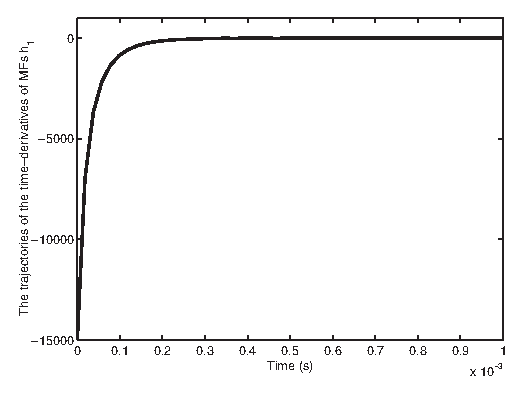
\includegraphics{fig1.eps}}
\caption{Chained interconnection topology with and without a leader\label{fig1}}
\end{figure}

\begin{table}[!t]
\processtable{Mobile robot parameters\label{tab1}}
{\begin{tabular}{@{\extracolsep{\fill}}lllll}\toprule
& & & Pioneer 2DX \\
Parameters & Pioneer 3DX & Pioneer 2DX & with load (4\,Kg) & Units\\\midrule
$\vartheta_{1}$ & \phantom{$-$}0.24089 & \phantom{$-$}0.3037 & \phantom{$-$}0.1992 & s \\
$\vartheta_{2}$ & \phantom{$-$}0.2424 & \phantom{$-$}0.2768 & \phantom{$-$}0.13736 & s \\
$\vartheta_{3}$ & $-$9.3603e$^{-4}$ & $-$4.018e$^{-4}$ & $-$1.954e$^{-3}$ & s.m/rad$^{2}$ \\
$\vartheta_{4}$ & \phantom{$-$}0.99629 & \phantom{$-$}0.9835 & \phantom{$-$}0.9907 \\
$\vartheta_{5}$ & $-$3.7256e$^{-3}$ & $-$3.818e$^{-3}$ & $-$1.554e$^{-2}$ & s/m \\
$\vartheta_{6}$ & \phantom{$-$}1.0915 & \phantom{$-$}1.0725 & \phantom{$-$}0.9866\\\botrule
\end{tabular}}{}
\end{table}

\begin{figure}[!t]
\centering{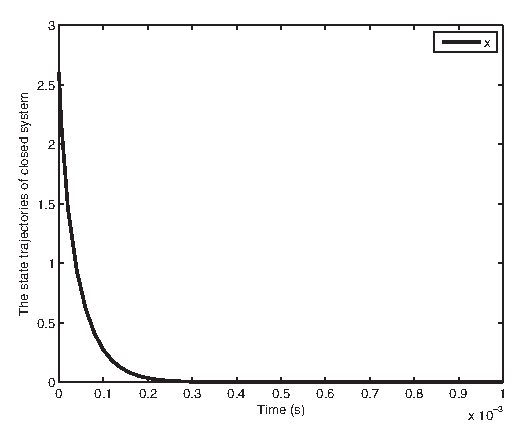
\includegraphics{fig2.eps}}
\caption{Consensus of trajectories of agents without a leader
\figfooter{a}{$\cos({\rm t})\omega_1=0.5$}
\figfooter{b}{$\omega_1=0$
{\rm Initial conditions and other parameters are chosen as $(p_i(0),q_i(0))=(0.2i,0.3i)$,
$c_{ij}=c_{ji}=0.2(i+j)$ and $m_i=0.1i (i,j=1,2,\ldots,6)$.}}
\label{fig2}}
\vskip-5pt
\end{figure}

\begin{corollary}\label{cor2}
Assume $b_{\rm L}(t)=b_{\rm L}$, $f(q_{\rm L})=q_{\rm L}(t)$ and suppose that the leader has
a path to all agents in graph $\mathcal{G}$. Then, $p_{i}(t)\rightarrow
p_{\rm L}(0)+{q_{\rm L}(0)}/{b_{\rm L}}$ as $t\rightarrow
+\infty$, where $p_{\rm L}(0)$ and $q_{\rm L}(0)$ are the initial position
and velocity of the leader, respectively.

\begin{proof}
If letting $b_{\rm L}(t)=b_{\rm L}$, $f(q_{\rm L})=q_{\rm L}(t)$,
then the solution of (\ref{eq4}) is given by
\vspace*{-2pt}\begin{align*}
p_{\rm L}(t)&=p_{\rm L}(0)+\frac{q_{\rm L}(0)}{b_{\rm L}}-\frac{q_{\rm L}(0)}{b_{\rm L}}\exp(-b_{\rm L}t)\\
q_{\rm L}(t)&=q_{\rm L}(0)\exp(-b_{\rm L}t)
\vspace*{-2pt}\end{align*}
so $p_{i}(t)\rightarrow
p_{\rm L}(0)+{q_{\rm L}(0)}/{b_{\rm L}}$ as $t\rightarrow+\infty$.
\end{proof}
\end{corollary}

\begin{figure}[!t]
\centering{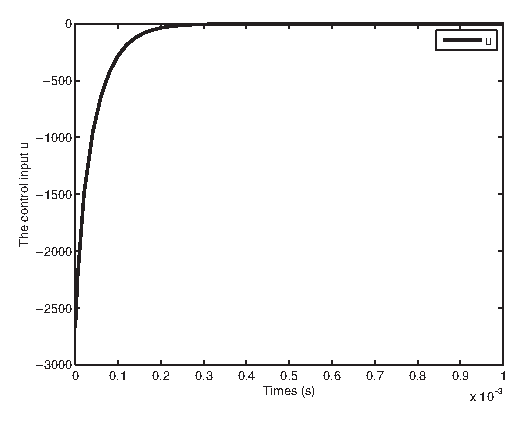
\includegraphics{fig3.eps}}
\caption{Consensus of trajectories of agents with a leader
\figfooter{a}{$d_L(t)=0.6+0.15\cos(t),\omega_2=0.5$}
\figfooter{b}{$b_L=0.6, \omega_2=0$\newline
{\rm Initial conditions and other parameters are chosen as $(p_i(0),q_i(0))=(-0.3i,0.4i)$,
$(p_L(0),q_L(0))=(1,0.3)$, $c_{ij}=c_{ji}=0.3(i+j)$, $b_i(t)=0.2i+0.15\cos(t),\omega_1=0.5$, $c_{1L}=1$
and $m_i=m_L=1$ $(i,j=1,2,\ldots,5)$.}}
\label{fig3}}
\end{figure}

\begin{remark}\label{rem3}
\looseness-1Protocol (3) contains a leader, which
provides the information to other agents and does not receive any
information from other agents. In protocol (3), the second term on
the right hand side of $u_{i2}(t)$ suggests that the leader has
relationships with some of the other agents in the group. In
particular, if for any $i\in\bar{N}$, $c_{i{\rm L}}>0 $, then the leader
has connections with all other agents. If for a specific agent $r$ and
$c_{rL}>0$, $c_{i{\rm L}}=0$ ($i\in\bar{N}, i\neq r$), then the leader has
a connection with one agent in the group. Since the leader has
a path to all other agents in graph $\mathcal{G}$, at least one agent can directly
receive information from the leader, and the other agents receive
information from the others either directly or indirectly. Theorem 2
also confirms that control of one agent in the group can ensure all
agents to achieve a desired consensus value provided that the graph
$\mathcal{G}$ is connected .
\end{remark}

\section{Numerical simulations}\label{sec4}

In order to illustrate the theoretical results, numerical
simulations were carried out for the system consisting of six
($N=6$, $n=1$) non-identical agents with and without a leader, as
shown in Fig.~\ref{fig1}. In the leaderless case, the non-linear control
protocols can be selected as
\begin{align}
u_{i1}(t) &= -b_{i}(t) f(q_{i}),\notag\\
u_{i2}(t)&=\sum_{j \in
\mathcal{N}_{i}}c_{ij} \,(p_{j}(t)-p_{i}(t))+\sum_{j \in
\mathcal{N}_{i}}c_{ij}(p_{j}(t)-p_{i}(t))^{3}\label{eq9}
\end{align}
and in the presence of a leader, the control protocols can be chosen as
\begin{align}
u_{i1}(t)&=-b_{i}(t)f(q_{i}),\notag\\
u_{i2}(t)&=\sum_{j\in\mathcal{N}_{i}}c_{ij}
(p_{j}(t)-p_{i}(t)+(p_{j}(t)-p_{i}(t))^{3})\notag\\
&\quad +c_{i{\rm L}}\, (p_{\rm L}(t)-p_{i}(t)+(p_{\rm L}(t)-p_{i}(t))^{3})\label{eq10}
\end{align}
where $f(q_{i})=q_{i}(t)+\omega_{1}\sin(q_{i})$ and
$f(q_{\rm L})=q_{\rm L}(t)+\omega_{2} \sin(q_{\rm L})\break (\omega_{1}\geq 0,
\omega_{2}\geq 0)$.

Fig.~\ref{fig2} shows the consensus process of positions and velocities of all agents in
system (1) with protocol (9). It indicates that all non-identical agents can achieve consensus
within a short period of time. From the result of
Corollary~1, the consensus value is found to be
${1}/{4.2}\sum_{i=1}^{6}(b_{i}p_{i}(0)+m_{i}q_{i}(0))\approx 1.5167$ as
$t\rightarrow +\infty$ when $b_{i}(t)=0.2i$, $m_{i}=0.1i$ and
$f(q_{i})=q_{i}(t)$. Fig.~\ref{fig3} illustrates that all positions and
velocities of system (1) with protocol (10) can track the position
and velocity of the leader. When $b_{\rm L}=0.6$, $f(q_{\rm L})=q_{\rm L}(t)$,
the exact position of the leader is
$p_{\rm L}(0)+{q_{\rm L}(0)}/{b_{\rm L}}=1.5$ as $t\rightarrow +\infty$ from
Corollary 2. It can be concluded from Figs.~\ref{fig2} and \ref{fig3} that the
theoretical results are in good agreement with numerical simulations.

\section{Conclusion}\label{sec5}

The consensus of multiple non-identical agents with \hbox{non-linear}
control protocols has been studied for the agents with and without a
leader. It was shown that all different agents in the group can
achieve consensus, and an explicit consensus value for the group was
obtained for some cases. For the agents with a leader, it was found
that all agents can track the position and velocity of the leader,
which are distinct from those of any follower agents. Numerical
simulations were used to illustrate the theoretical results.

\section{Acknowledgments}

Shan Cheng is indebted to the China Scholarship Council (CSC)
for its financial support as a visiting scholar at the University of
Technology, Sydney. This work was partially supported by the
National Science Foundation of China (Grant no. 10972129), the
Innovation Program of Shanghai Municipal Education Commission (Grant
no. 10ZZ61), the Shanghai Leading Academic Discipline Project (Project no.
S30106), and the Graduate Innovation Foundation of Shanghai
University (Project no. SHUCX 101080).

\begin{thebibliography}{99}

\bibitem{1}
Vicsek T., Czir\'{o}k A., Ben-Jacob E., Cohen I.: `Novel type of phase transition in a system of self-driven particles', \textit{Phys. Rev. Lett.}, 1995, \textbf{75}, pp.~1226--1229

\bibitem{2}
Jadbabaie A., Lin J., Morse A.S.: `Coordination of groups of
mobile autonomous agents using nearest neighbor rules', \textit{IEEE
Trans. Autom. Control}, 2003, \textbf{48}, pp.~988--1001

\bibitem{3}
Olfati-Saber R., Murray R.M.: `Consensus problems in networks
of agents with switching topology and time-delays', \textit{IEEE Trans.
Autom. Control}, 2004, \textbf{49}, pp.~1520--1533

\bibitem{4}
Ren W., Atkins E.: `Distributed multi-vehicle coordinated
control via local information exchange', \textit{Int. J. Robust
Nonlinear Control}, 2007, \textbf{17}, pp.~1002--1033

\bibitem{5}
Ren W.: `On consensus algorithms for double-integrator dynamics',
\textit{IEEE Trans. Autom. Control}, 2008, \textbf{53}, pp.~1503--1509

\bibitem{6}
Xie G., Wang L.: `Consensus control for a class of networks of
dynamic agents', \textit{Int. J. Robust Nonlinear Control}, 2007,
\textbf{17}, \hbox{pp.~941--959}

\bibitem{7}
Gao Y., Wang L.: `Consensus of multiple dynamic agents with sampled information', \textit{IET Control
Theory Appl.}, 2010, \textbf{4}, pp.~945--956

\bibitem{8}
Tanner H.G., Jadbabaie A., Pappas G.J.: `Flocking in fixed
and switching networks', \textit{IEEE Trans. Autom. Control}, 2007,
\textbf{52}, \hbox{pp.~863--868}

\bibitem{9}
Lee D.J., Spong M.W.: `Stable flocking of multiple inertial
agents on balanced graphs', \textit{IEEE Trans. Autom. Control}, 2007,
\textbf{52}, \hbox{pp.~1469--1475}

\bibitem{10}
Hu J., Lin Y.S.: `Consensus control for multi-agent systems with double-integrator dynamics and time delays', \textit{IET Control
Theory Appl.}, 2010, \textbf{4}, pp.~109--118

\bibitem{11}
Lin P., Jia Y.: `Further results on decentralised coordination
in networks of agents with second-order dynamics', \textit{IET Control
Theory Appl.}, 2009, \textbf{3}, pp.~957--970

\bibitem{12}
Lin P., Jia Y.: `Robust $H_{\infty}$ consensus analysis of a class of second-order multi-agent systems with uncertainty', \textit{IET Control
Theory Appl.}, 2010, \textbf{4}, pp.~487--498

\bibitem{13}
He W., Cao J.: `Consensus control for high-order multi-agent
systems', \textit{IET Control Theory Appl.}, 2011, \textbf{1}, pp.~231--238

\bibitem{14}
Hui Q., Haddad W.M.: `Distributed nonlinear control algorithms
for network consensus', \textit{Automatica}, 2008, \textbf{44}, pp.~2375--2381

\bibitem{15}
Liu X., Chen T., Lu W.: `Consensus problem in directed
networks of multi-agents via nonlinear protocols', \textit{Phys. Lett.
A}, 2009, \textbf{373}, pp.~3122--3127

\bibitem{16}
Zheng Y., Zhu Y., Wang L.: `Consensus of heterogeneous multi-agent systems', \textit{IET Control
Theory Appl.}, 2011, \textbf{5}, pp.~1881--1888

\bibitem{17}
Zhang W., Zeng D., Qu S.: `Dynamic feedback consensus control of a class of high-order multi-agent systems',
\textit{IET Control Theory Appl.}, 2010, \textbf{4}, pp.~2219--2222

\bibitem{18}
Su H.S., Wang X.F., Lin Z.L.: `Flocking of multi-agents with
a virtual leader', \textit{IEEE Trans. Autom. Control}, 2009,
\textbf{54}, pp.~293--307

\bibitem{19}
Song Q., Cao J., Yu W.: `Second-order leader-following
consensus of nonlinear multi-agent system via pinning control', \textit{Syst. Control Lett.}, 2010, \textbf{59}, pp.~553--562

\bibitem{20}
Hong Y.G., Chen G.R., Bushnell L.D.: `Distributed observers
design for leader-following control of multi-agent networks', \textit{Automatica}, 2008, \textbf{44}, pp.~846--850

\bibitem{21}
Hu J., Hong Y.: `Leader-following coordination of multi-agent
systems with coupling time delays', \textit{Physica A}, 2007,
\textbf{374}, pp.~853--863

\bibitem{22}
Ren W.: `Consensus strategies for cooperative control of vehicle
formations', \textit{IET Control Theory Appl.}, 2007, \textbf{1}, pp.~505--512

\bibitem{23}
Khalil H.K.: `Nonlinear systems' (Prentice-Hall, New
Jersey,  2002, 3rd edn.)

\end{thebibliography}

\end{document}
